\documentclass[a4paper,11pt]{article}
\usepackage[utf8]{inputenc}
\usepackage{amsmath}
\usepackage{amsfonts}
\usepackage{amssymb}
\usepackage{graphicx}
\usepackage{tabularx}
\usepackage[font=scriptsize]{caption}
\usepackage[font=scriptsize]{subcaption}
\usepackage{wrapfig}
\usepackage[backend=biber]{biblatex}

\addbibresource{nn.bib}
\renewcommand\thesubsection{\alph{subsection}}


%opening
\title{A population firing rate encoder based on cortical minicolumns}
\author{Vince Baker, advisor: Dr. Luis Cruz Cruz\\ Drexel University Department of Physics}

\begin{document}

\maketitle

\begin{abstract}
We propose a neural circuit topology to encode population firing rate information.
The topology is based on the observed minicolumn structure found in the mammalian cortex.
The proposed neural circuit provides a strong, sparse encoding of peaks in the population firing rate through synchronized traveling waves in the minicolumn structures.
\end{abstract}

\section{Introduction} 
Information in the brain is encoded by the firing rates of neurons.
Individual neurons in the brain do not reliably respond to a specific stimulus in a consistent manner.
A stimulus may, however, be reliably encoded in the average firing rate of a pool of neurons with similar tuning \cite{trappenberg}.

The mammalian cortex has a laminar structure segmented into layers \cite{banich}.
Perpendicular to these layers are vertical units of organization called minicolumns or microcolumns that travers layers II through VI \cite{buxhoeveden2002}\cite{cruz2005}.
These minicolumns are about 30-50 $\mu$m wide and contain about 100 neurons.
Although this minicolumn organization was observed decades ago the functional purpose of minicolumns, if any, remains unclear \cite{horton2005}.

Neurons in the cortex are dominated by local connectivity, such that neurons are most strongly connected to nearby neurons \cite{levy2012}.
Locally connected neurons can spread their firings to neighboring neurons creating what has been called a travelling wave of neuron activation. 
These travelling waves in locally connected networks have been observed in the cortex of mammalian brains as well as in vitro, and subsequently have been reproduced in silico \cite{keane2015}\cite{ermentrout2001}\cite{wu2008}.
Cortical traveling waves have been observed on multiple spatial and temporal scales, and a number of functional roles have been proposed \cite{muller2018}.

We propose a neural circuit to encode the firing rate of a population of neurons.
The proposed circuit is composed of locally connected neurons arranged in minicolumns.
A pool of input neurons is connected to the base of the minicolumns.
Peaks in the population firing rate of the input pool evoke traveling waves that travel up the minicolumns.
These traveling waves produce a strong, sparse representation at the top of the minicolumns.
We observe that weakly connected minicolumns produce the most reliable, clean and efficient encoding.

\section{Methods}
Neuron and synapse dynamics, single column model
\\ \\
Minicolumn ensembles (one big column, weakly connected columns, disconnected minicolumns)
\\ \\
The input to our system is generated from a pool of 50 neurons with a common instantaneous firing rate.
We use a raised-cosine function for the firing rate input.
Each input neuron is connected to every excitatory neuron at the base layer of the minicolumn ensemble with a probability of connection of $50\%$ and a connection strength of $5/2$. 
The input neurons have a common firing rate that varies over time.
For each $10 ms$ time window a Poisson spike train of duration $10 ms$ is generated for every input neuron based on the instantaneous firing rate.
The output from each neuron in the input pool is calculated by convolving the neuron's spike train with an exponential synaptic response $e^{(t-t^f)/\sigma}$ where $t^f$ is the neuron firing time and $\sigma = 4ms$.
The input signal to each neuron in the base layer of the minicolumn ensemble is summed from the input pool stimulus according to the synaptic connections (Figure \ref{fig:firingrate_input}).

\begin{figure}[!ht]
 \caption{Firing rate input. The instantaneous firing rate (top) is encoded into spike trains of a pool of 50 neurons (middle), generating a stimulus to the base layer of the minicolumn ensemble (bottom). The stimulus at the bottom is shown as a membane potential in mV.}
 \label{fig:firingrate_input}
 \centering
   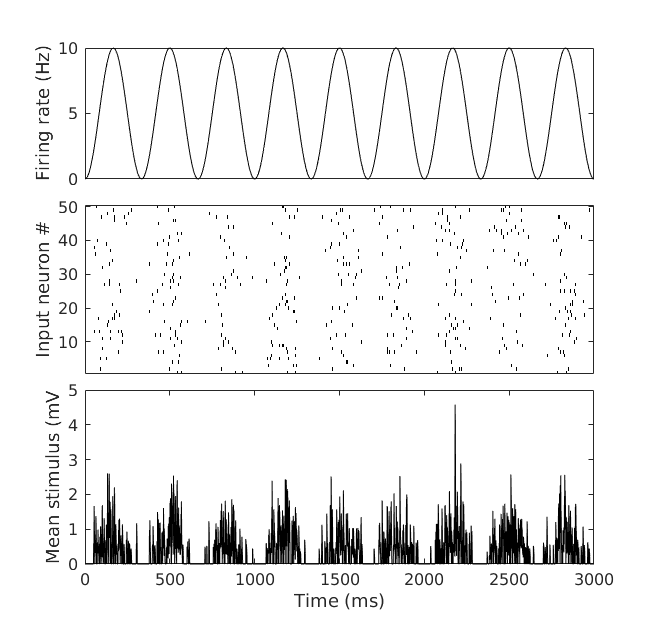
\includegraphics[width=0.75\textwidth]{fig/InputFiringRate}
\end{figure}

All neurons in the neural circuit also receive a background stimulus representative of noise.

\begin{figure}[!ht]
 \caption{The neural circuit is stimulated by the pool of input neurons at the base layer. The output is taken as the mean membrane potential at the top layer. Information is transmitted up the minicolumns via traveling waves. }
 \label{fig:system_diagram}
 \centering
   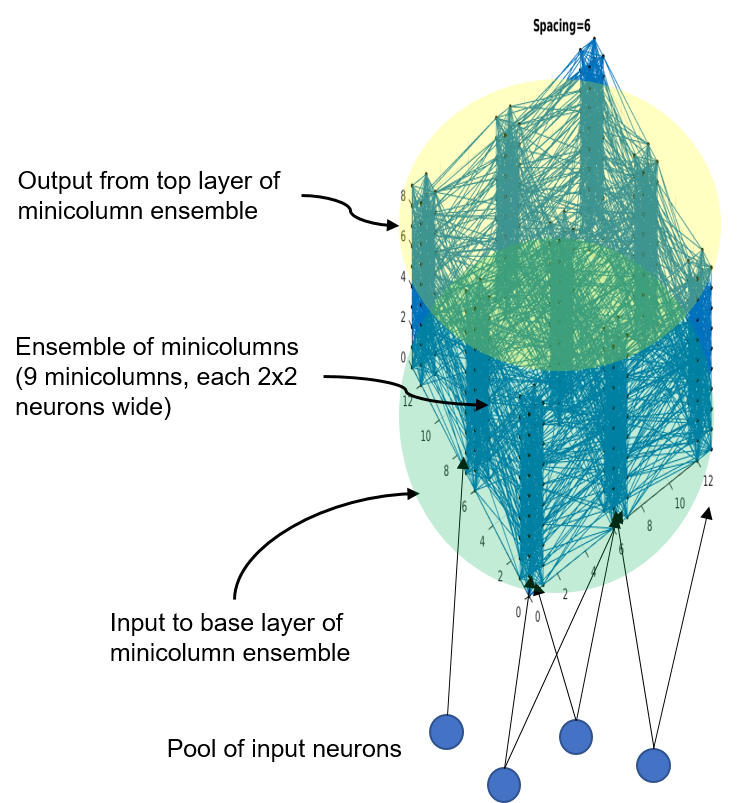
\includegraphics[width=0.5\textwidth]{fig/SystemDiagram}
\end{figure}

The system output is taken as the average membrane potential of the neurons in the top layer of the minicolumn ensemble.
We expect the population mean membrane potential to exhibit similar characteristics to an individual neuron \cite{trappenberg}.
We therefore characterize the spiking behavior of the output by peaks in the membrane potential.

The spikes in the population membrane potential have a similar shape to an individual neuron spike, with a sharp increase in potential (depolarization) followed by a refractory period below the resting potential (hyperpolarization).
To locate and characterize the spikes we first remove the refractory periods by clipping the output below $-68\ mV$, our average resting potential.
We then add $68\ mV$ to the output to shift the base to zero.
We use a peak detection threshold of $25\%$ of the maximum value in the output data.
The peak locations and peak widths are then extracted from the data (Figure \ref{fig:peak_det}).

The accuracy of the encoding is measured from the peaks in the output through a peak number error $\kappa$ and a peak position error $\pi$.
$\kappa$ is the difference in the number of peaks detected in the output and the number of peaks in the input firing rate.
$\pi$ is the difference in milliseconds between the peak position and the closest peak in the firing rate input.

\begin{figure}[!ht]
 \caption{Illustration of the peak detection. The original output is shown on the left. The data on the right (blue) after removing the refractory period and shifting by $68\ mV$, with a $10\%$ threshold (red). }
 \label{fig:peak_det}
 \centering
   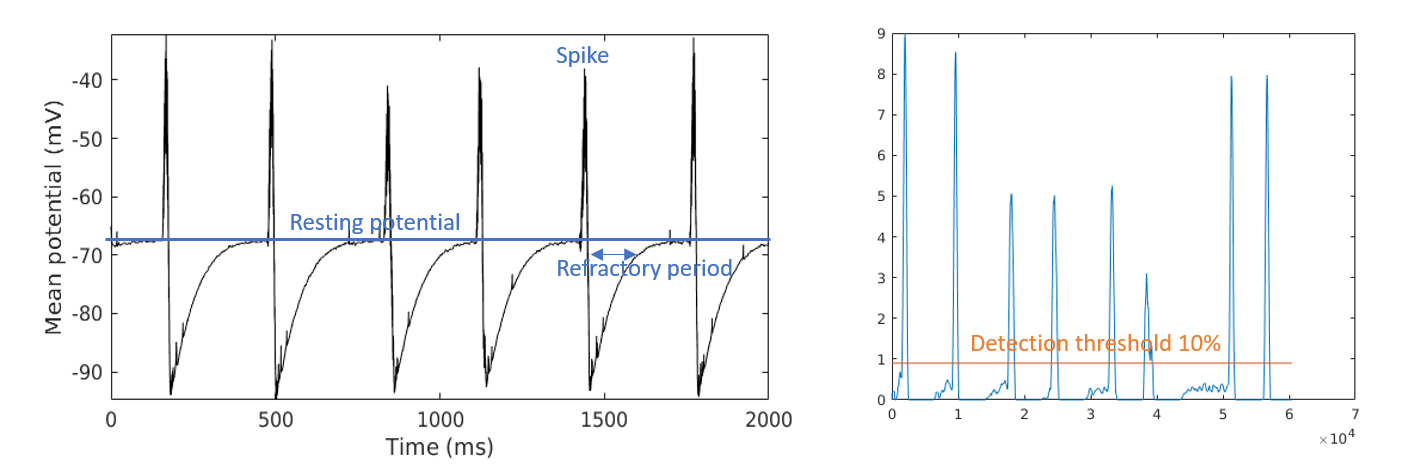
\includegraphics[width=\textwidth]{fig/PeakDetectionExample}
\end{figure}


\clearpage
\section{Results}
Our basic circuit is an ensemble of nine minicolumns. 
Each minicolumn is 2x2x20 neurons. 
We vary the separation between adjacent columns to acheive different degrees of connectivity.

We observe traveling waves in the minicolumns as illustrated in Figure \ref{fig:firing_video} (full videos online).
The stimulus-evoked traveling waves reliably traverse the minicolumns from bottom to top.
We also observe some traveling waves initiated by the background noise.
These spontaneous traveling waves can start from anywhere in the minicolumns, and will spread both up and down from the point of origin.
\begin{figure}[!ht]
 \caption{Three frames of a simulation showing all neurons in the circuit. Colors represent the neuron membrane potential. The traveling waves are initiated at the base of the circuit (left), propoagate upward (center) and terminate at the top (right).} 
 \label{fig:firing_video}
 \centering
   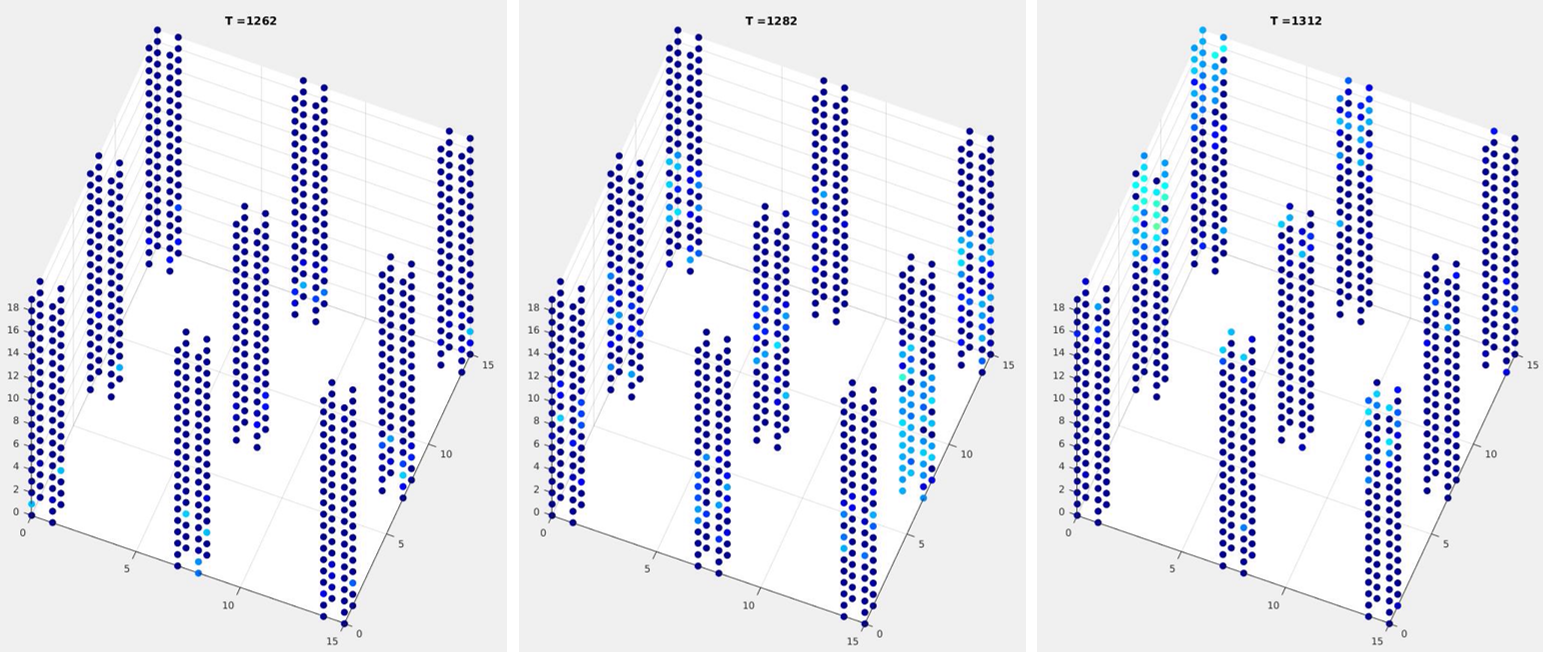
\includegraphics[width=\textwidth]{fig/VideoStills}
\end{figure}

We observe strong correlation between input firing rate fluctuation and the output of the minicolumn ensemble.
\begin{figure}[!h]
 \caption{The input stimulus (top) is quite noisy and diffuse. The minicolumn ensemble encodes the input into a sequence of strong, clean spikes (bottom).}
 \label{fig:goodIO}
 \centering
   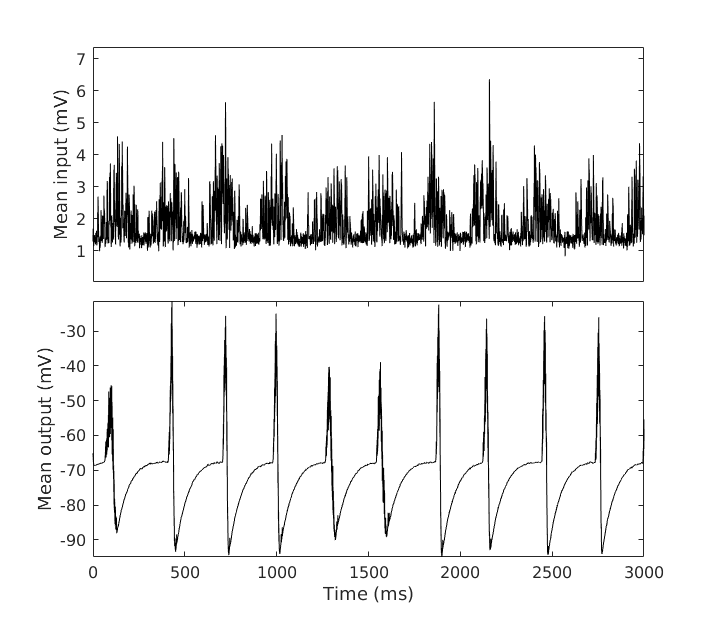
\includegraphics[width=0.75\textwidth]{fig/InputOutput_Sep7}
\end{figure}

We measured $\kappa$ and $\pi$ for minicolumn ensembles with inter-column spacing from 4 to 20.
The columns were constructed of identical neurons.
The change in spacing alters the inter-column connectivity and action potential propagation time.
We found that the more highly connected minicolumn ensembles encode the input firing rate with lower error (Figure \ref{fig:encoding_results}).
Minicolumn ensembles with moderate connectivity accurately encoded the population firing rate of the pool of input neurons.
Less connected ensembles showed less synchronization in the output, with traveling waves in the individual minicolumns arriving at different times.
Very highly connected ensembles (separation 3) 

\begin{figure}[!ht]
 \caption{Firing rate encoding error for minicolumn ensembles of different inter-column spacing. The RMS errors are shown for $\kappa$ (number of peaks) and $\pi$ (peak position).}
 \label{fig:encoding_results}
 \centering
   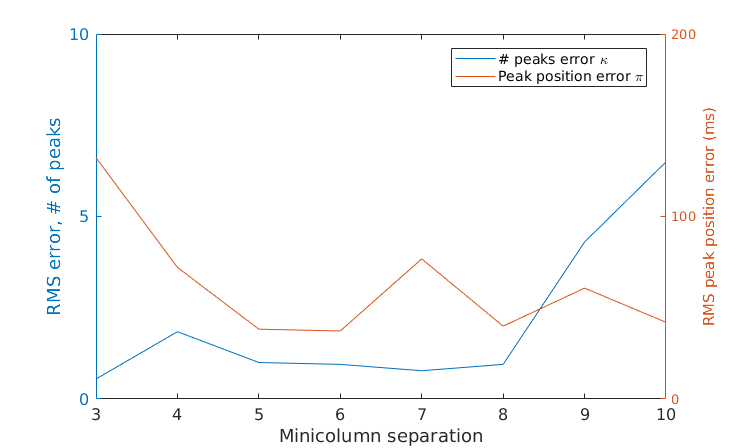
\includegraphics[width=0.75\textwidth]{fig/EncodingError_10Trials}
\end{figure}

Minicolumn ensembles close inter-column spacing (2-4 units) do not effectively encode the firing rate information.
With spacing of 2 units the entire ensemble is rapidly consumed with firing activity.
Figure \ref{fig:onebigcolumn} shows the firting events per neuron in such a system.
After a short time all neurons in the ensemble are highly active with no discernible pattern in the firing activity.
\begin{figure}[!ht]
 \caption{Neuron firing events in a fully connected ensemble with column separation of 2 units.} 
 \label{fig:onebigcolumn}
 \centering
   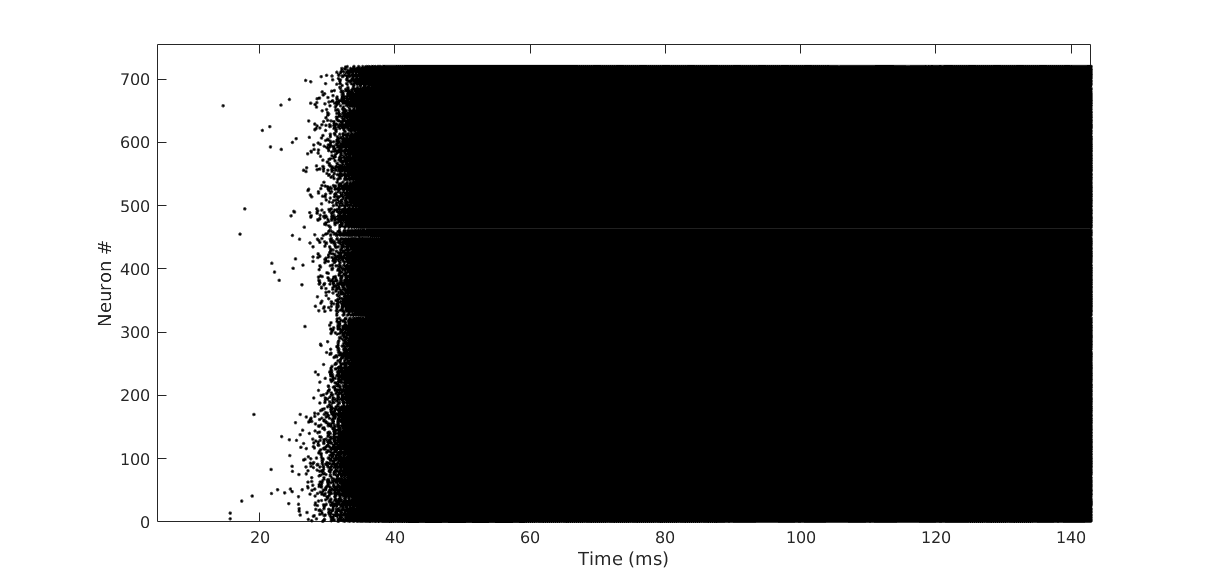
\includegraphics[width=\textwidth]{fig/OneBigColumn}
\end{figure}


\clearpage
\section{Discussion}
We have demonstrated a neural circuit for encoding the firing rate of a population of neurons into a strong, clean signal.
The proposed neural circuit is inspired by the minicolumn structures found in the mammalian cortex, and could represent a functional role for this type of morphology.


\clearpage
\printbibliography

\end{document}
